% !TeX root = mos-en.tex

%%%%%%%%%%%%%%%%%%%%%%%%%%%%%%%%%%%%%%%%%%%%%%%%%%%%%%%%%%%%%

\begin{center}
\textbf{\LARGE Problems and solutions}
\end{center}

\addcontentsline{toc}{section}{\large Problems and solutions}

\begin{prob}{The sock drawer}
A drawer contains red and black socks. If two socks are drawn at random without replacement the probability that both are red is $\frac{1}{2}$. 

\que{1} How small can the number of black socks in the drawer be? What is the corresponding number of red socks?

\que{2} How small can the number of black socks in the drawer be if the number of black socks is \emph{even}? What is the corresponding number of red socks?
\end{prob}

\solution{1}

\ans{1} Let $r$ be the number of red socks in the drawer and let $b$ the number of black socks.  $r\geq 2$ since two red socks are drawn and $b\geq 1$ since otherwise the probability of drawing two red socks would be $1$.

Multiplying the probabilities for the two draws gives:
\begin{equation}\label{eq.1-a}
P(\textsf{two red})=\frac{r}{r+b} \cdot \frac{(r-1)}{(r-1)+b} = \frac{1}{2}\,.
\end{equation}
Simplifying results in a quadratic equation in the variable $r$:
\begin{equation}\label{eq.quad-for-r}
r^2-r(2b+1)-(b^2-b)=0\,.
\end{equation}
Since $r,b$ are positive integers the discriminant must be the square of an integer:
\begin{equation}\label{eq.discriminant}
(2b+1)^2+4(b^2-b)=8b^2+1
\end{equation}
The discriminant is a square when $b=1$ (its smallest value). From Equation~\ref{eq.quad-for-r}, $r=3$ where we reject the solution $r=0$ because $r\geq 2$. The total number of socks is $4$.

Check: $\frac{3}{4}\cdot\frac{2}{3}=\frac{1}{2}$.

\medskip

\ans{2}
Check positive even values of $b$ to find the smallest one for which the discriminant is a square:
\begin{displaymath}
\renewcommand{\arraystretch}{1}
\begin{array}{r|r|r}
b&8b^2+1&\sqrt{8b^2+1}\\
\hline
2&33&5.74\\
4&129&11.36\\
\mathbf{6}&\mathbf{289}&\mathbf{17}
\end{array}
\end{displaymath}
For $b=6$ the corresponding value for $r$ is $15$.

Check: $\frac{15}{21}\cdot\frac{14}{20}=\frac{1}{2}$.

\newpage

\solution{2}

\ans{1}
Is the following inequality is true?
\begin{equation}\label{eq.1-b}
\frac{r}{r+b} \stackrel{?}{>} \frac{r-1}{(r-1)+b}\,.
\end{equation}
$r\geq 2, b\geq 1$, so both denominators are positive and we can multiply the two sides:
\begin{eqn}
r(r-1+b)&\stackrel{?}{>}&(r-1)(r+b)\\
r^2-r+rb&\stackrel{?}{>}&r^2-r+rb-b\\
b&\stackrel{?}{>}&0\,.
\end{eqn}%
$b>1$ so Equation~\ref{eq.1-b} is true.

By Equations~\ref{eq.1-a}, \ref{eq.1-b}:
\begin{equation}\label{eq.1-c}
\left(\frac{r}{r+b}\right)^2 = \frac{r}{r+b} \cdot\frac{r}{r+b} > \frac{r}{r+b} \cdot \frac{r-1}{(r-1)+b} = \frac{1}{2}\,,
\end{equation}
and similarly:
\begin{equation}\label{eq.1-d}
\left(\frac{r-1}{(r-1)+b}\right)^2  = \frac{r-1}{(r-1)+b}\cdot \frac{r-1}{(r-1)+b}<  \frac{r}{r+b} \cdot \frac{r-1}{(r-1)+b} = \frac{1}{2}\,.
\end{equation}
$r+b$ is non-zero so we can take the square root of Equation~\ref{eq.1-c} and simplify:
\begin{eqn}
\frac{r}{r+b}  &>& \sqrt{\frac{1}{2}}\\
r&>&\frac{b}{\sqrt{2}-1}=\frac{b}{\sqrt{2}-1}\cdot\frac{\sqrt{2}+1}{\sqrt{2}+1}\\
r&>&b(\sqrt{2}+1)\,.
\end{eqn}%
Similarly for Equation~\ref{eq.1-d}:
\begin{eqn}
\frac{r-1}{(r-1)+b}&<&\sqrt{\frac{1}{2}}\\
r-1 &<& \frac{b}{\sqrt{2}-1}\\
r-1&<&b(\sqrt{2}+1)\,.
\end{eqn}%
Combining both equations we get:
\begin{equation}\label{eq.inequalities}
r-1<(\sqrt{2}+1)b<r\,.
\end{equation}
For $b=1$ we have $2.141 < r< 3.141$ and $b=1,r=3$ is a solution.

\ans{2} Check positive even values of $b$:
\begin{displaymath}	
\renewcommand{\arraystretch}{1}
\begin{array}{r|ccc|c|c}
b& (\sqrt{2}+1)b&<r<& (\sqrt{2}+1)b+1&r&P(\textrm{two reds})\\
\hline
2&4.8&<r<&5.8&5&0.4762\\
4&9.7&<r<&10.7&10&0.4945\\
6&14.5&<r<&15.5&
15&0.5000
\end{array}
\end{displaymath}
Mosteller mentions a connection between this problem and advanced number theory, and gives another solution: $b=35,r=85$.

\medskip
\sml{}
\begin{verbatim}
Expectation of both red  = 0.5000
Average of both red for (red =  3, black =  1) = 0.5053
Average of both red for (red = 15, black =  6) = 0.5013
Average of both red for (red = 85, black = 35) = 0.4961
\end{verbatim}

\textbf{Comment}

Neither solution provides a \emph{sufficient} condition for the values of $r,b$. In Solution~1 we derive a necessary condition---by Equation~\ref{eq.discriminant} the discriminant must be an integer---and start searching for values of $b$ that satisfy this requirement. In Solution~2 the necessary condition is that $r,b$ must satisfy the inequalities in Equation~\ref{eq.inequalities} and then we search for values that satisfy the requirement that the probability of two reds must be $0.5$.

I wrote a program to search for solutions. For $r$ near $35$:
\[
\renewcommand{\arraycolsep}{12pt}
\begin{array}{r|r|r|r}
\multicolumn{1}{c|}{r}&
\multicolumn{1}{c|}{b}&
\multicolumn{1}{c|}{\sqrt{8b^2+1}}&
\multicolumn{1}{c}{P(\textsf{two red})} \\\hline
32 & 78  & 90.52 & 0.500917\\
33 & 80  & 93.34 & 0.499368\\
34 & 83  & 96.17 & 0.501474\\
35 & 85  & 99.00 & 0.500000\\
36 & 87  &101.83 & 0.498601\\
37 & 90  &104.66 & 0.500562
\end{array}
\]
Here are the solutions for $b<10^6$:
\[
\begin{array}{r@{\hspace{2em}}r}
\textsf{black} & \textsf{red}\\\hline
1 & 3 \\
6 & 15\\
35 &  85\\
204 &  493\\
1189 &  2871\\
6930 & 16731\\
40391 &  97513\\
235416 & 568345
\end{array}
\]

%%%%%%%%%%%%%%%%%%%%%%%%%%%%%%%%%%%%%%%%%%%%%%%%%%%%%%%%%%%%%

\begin{prob}{Successive wins}
You play a sequence of three games alternately against two players and you win the sequence if you win at least two of the three games \emph{in a row}. The probability that you will win a game against player $P_1$ is $p_1$ and the probability that you will win a game against player $P_2$ is $p_2$. It is given that $p_1>p2$. Which of these sequences gives you a better chance of winning?
\begin{itemize}
\item You play against $P_1,P_2,P_1$ in that order.
\item You play against $P_2,P_1,P_2$ in that order.
\end{itemize}
\end{prob}

\solution{1}

You win if: (a) you win the first two games and lose the last game, (b) you lose the first game and win the last two games, or (c) you win all three games.

Let $p_{121}$ be the probability that you win with the sequence $P_1,P_2,P_1$ and let $p_{212}$ be the probability that you win with the sequence $P_1,P_1,P_2$. Then:
\begin{eqn}
p_{121}&=&p_1p_2(1-p_1) + (1-p_1)p_2p_1 + p_1p_2p_1\\
p_{212}&=&p_2p_1(1-p_2) + (1-p_2)p_1p_2 + p_2p_1p_2\,.
\end{eqn}%
You have a better chance of winning with the sequence $P_1,P_2,P_1$ if $p_{121}>p_{212}$, that is, if:
\[
p_1p_2(1-p_1) + (1-p_1)p_2p_1 + p_1p_2p_1 \stackrel{?}{>} 
p_2p_1(1-p_2) + (1-p_2)p_1p_2 + p_2p_1p_2\,.
\]
Cancel $p_1p_2$ from all terms:
\begin{eqn}
(1-p_1)+(1-p_1)+p_1 & \stackrel{?}{>}& (1-p_2)+(1-p_2)+p_2\\
-p_1&\stackrel{?}{>}&-p_2\\
p_2&\stackrel{?}{>}&p_1\,,
\end{eqn}%
but by assumption $p_1>p_2$ so you should choose the sequence $P_2,P_1,P_2$,

\solution{2}

The result is counter-intuitive. Intuitively, you should choose to play two games with $P_1$ and one game with $P_2$ because more likely to win games against $P_1$. However, the only way that you can win the sequence is by winning the \emph{middle} game, and, therefore, you should play the middle game against $P_1$, the player you are more likely to defeat.

\newpage

\sml{}
\begin{verbatim}
For p1 = 0.6, p2 = 0.5
Proportion of P121 wins = 0.4166
Proportion of P212 wins = 0.4473

For p1 = 0.6, p2 = 0.4
Proportion of P121 wins = 0.3300
Proportion of P212 wins = 0.3869

For p1 = 0.6, p2 = 0.2
Proportion of P121 wins = 0.1625
Proportion of P212 wins = 0.2141
\end{verbatim}

%%%%%%%%%%%%%%%%%%%%%%%%%%%%%%%%%%%%%%%%%%%%%%%%%%%%%%%%%%%%%

\begin{prob}{The flippant juror}
There are two options to reach a decision: (a) A three-person panel consisting of two members who independently make the correct decision with probability $p$ and one member who makes the correct decision with probability $1/2$. The final decision is determined by a majority vote. (b) A one-person panel whose only member has probability $p$ of making the correct decision. Which option has the higher probability of making the correct decision?
\end{prob}

\solution{}

The three-person panel makes the correct decision if all three members make the correct decision or if any subset of two members makes the correct decision:
\[
P(\textsf{correct decision})=\overbrace{\left(p\cdot p\cdot\frac{1}{2}\right)}^{\textsf{all three correct}}+\;\;\overbrace{\left(p(1-p)\cdot\frac{1}{2}+(1-p)p\cdot\frac{1}{2}+p\cdot p\cdot\frac{1}{2}\right)}^{\textsf{two out of three correct}}=p\,,
\]
so there is no difference between the two options.

\sml{}
\begin{verbatim}
Prediction: probabilities of (a) and (b) are equal
For p = 0.25, proportion correct of (a) = 0.5019, (b) = 0.5046
For p = 0.50, proportion correct of (a) = 0.5072, (b) = 0.4970
For p = 0.75, proportion correct of (a) = 0.5062, (b) = 0.5040
\end{verbatim}

%%%%%%%%%%%%%%%%%%%%%%%%%%%%%%%%%%%%%%%%%%%%%%%%%%%%%%%%%%%%%

\newpage

\begin{prob}{Trials until first success}
\label{p.four}
What is the expectation of the number of throws of a die until a $6$ appears?
\end{prob}

\solution{1}

The probability that the $i$th throw will be the first occurrence of $6$ is the probability of $i-1$ throws of one of the other five numbers times the probability that the $i$th throw will be $6$.

To simplify notation let $p=1/6$, $P=P(\textsf{first}\:6\:\textsf{on}\:i\textsf{th throw})$, $E=E(\textsf{first throw of}\:6)$. Then:
\begin{eqnlabels}
\nonumber{}P&=&(1-p)^{i-1}p\\
\label{eq.first-expec}E&=&1p(1-p)^0 + 2p(1-p)^1+ 3p(1-p)^2+ 4p(1-p)^3 +\cdots =\sum_{i=1}^{\infty} ip(1-p)^{i-1}\,.
\end{eqnlabels}
Without the factor $i$ the sum would be the probability of eventually throwing a $6$:
\begin{equation}\label{eq.geo}
P(\textsf{eventually throwing a}\;6)= \sum_{i=1}^{\infty} p(1-p)^{i-1}=p\cdot\frac{1}{1-(1-p)}=1\,,
\end{equation}
which is not a surprising result.

The calculation of the expectation can be performed as follows:
\[
\renewcommand{\arraycolsep}{2pt}
\begin{array}{lllllllllll}
E&\!\!=\!\!&p(1-p)^0 &+& p(1-p)^1&+& p(1-p)^2&+& p(1-p)^3 &+&\cdots \\
& & &&p(1-p)^1&+& p(1-p)^2&+& p(1-p)^3 &+&\cdots \\
&  &&&& &p(1-p)^2&+& p(1-p)^3 &+&\cdots \\
&&&&&&&&p(1-p)^3 &+&\cdots
\end{array}
\]
The first row is the sum of the geometric series from Equation~\ref{eq.geo} which is $1$. The second row is the same geometric series except that the first element is $p(1-p)$ so its sum is:
\[
\frac{p(1-p)}{1-(1-p)}=1-p\,.
\]
Similarly, the sum of the third row will be $(1-p)^2$ and the sum of the $i$th row will be $(1-p)^{i-1}$. Therefore, the expectation is the sum of the geometric series:
\[
E= 1 + (1-p) + (1-p)^2 + (1-p)^3 + \cdots= \frac{1}{1-(1-p)}=\frac{1}{p}=6\,.
\]

\solution{2}

Multiply Equation~\ref{eq.first-expec} by $1-p$ and subtract the result from that equation. The result is the geometric series in Equation~\ref{eq.geo}:
\[
\renewcommand{\arraycolsep}{2pt}
\begin{array}{rclllllllll}
E&=&p(1-p)^0 &+&2p(1-p)^1&+& 3p(1-p)^2&+& 4p(1-p)^3 &+&\cdots\\
E\cdot(1-p)&=&&&p(1-p)^1 &+& 2p(1-p)^2&+& 3p(1-p)^3 &+&\cdots \\
E\cdot(1-(1-p)) &=& p &+& p(1-p)^1 &+& p(1-p)^2 &+& p(1-p)^3 &+&\cdots\\
Ep&=&1\\
E&=&1/p=6\,.
\end{array}
\]

\solution{3}

Consider the first throw separately from the rest of the throws. If the first throw is a $6$ (probability $p$) then one throw is sufficient. Otherwise, if the first throw is not a $6$ (probability $1-p$), then the remaining throws form a sequence identical to the original one so the expectation of this sequence is $E$:
\begin{eqn}
E &=& 1p + (E+1)(1-p)\\
E&=&1/p=6\,.
\end{eqn}%

\sml{}
\begin{verbatim}
Expectation of first success = 6
Average of first success     = 6.0161
\end{verbatim}

%%%%%%%%%%%%%%%%%%%%%%%%%%%%%%%%%%%%%%%%%%%%%%%%%%%%%%%%%%%%%


\begin{prob}{Coin in a square}

A coin is thrown onto an (unbounded) grid of squares of uniform size. The position of the center of the coin is uniformly distributed within the square in which it lands.

\que{1} Given a square of side $8$ and a coin of radius $3$ what is the probability that the coin lands entirely within the square?

\que{2} For each throw you win $5$ if the coin lands within the square and lose $1$ if it touches a side of the square. What is the expectation of your winnings for each throw?

\que{3} Develop a formula for the probability of the coin landing within the square if the side of the square is $a$ and the radius of the coin is $r<a/4$.
\end{prob}

\solution{}

\ans{1} \ref{f.coins1} shows a square of side $8$ and four circles of radius $3$ inscribed within the corners of the square. The centers of the circles form an inner square of side $2$. Any coin whose center is outside the inner square will touch an edge of the outer square. Since the center of the coin is uniformly distributed, the probability that the coin lands entirely within the square is the ratio of the area of the inner square to the area of the outer square:
\[
P(\textsf{coin lands within the square})=\frac{2\cdot 2}{8\cdot 8} =\frac{1}{16}=0.0625\,.
\]
\begin{figure}[tb]
\begin{center}
\begin{subfigure}{.43\textwidth}
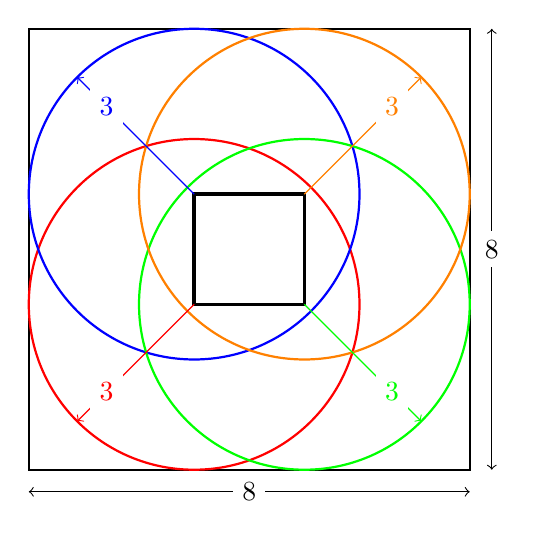
\begin{tikzpicture}[scale=.7]
\coordinate (c1) at (3,3);
\coordinate (c2) at (3,5);
\coordinate (c3) at (5,3);
\coordinate (c4) at (5,5);
\draw[very thick] (c1) -- (c3) -- (c4) -- (c2) -- cycle;
\draw[thick] (0,0) rectangle +(8,8);
\draw[color=red,thick] (c1) circle[radius=3];
\draw[color=blue,thick] (c2) circle[radius=3];
\draw[color=green,thick] (c3) circle[radius=3];
\draw[color=orange,thick] (c4) circle[radius=3];
\vertexcolor{c1}{red};
\vertexcolor{c2}{blue};
\vertexcolor{c3}{green};
\vertexcolor{c4}{orange};
\draw[<->] (0,-.4) -- node[fill=white] {$8$} (8,-.4);
\draw[<->] (8.4,0) -- node[fill=white] {$8$} (8.4,8);
\draw[->,red] (3,3) -- node[near end,fill=white] {$3$} +(-135:3);
\draw[->,blue] (3,5) -- node[near end,fill=white] {$3$} +(135:3);
\draw[->,green] (5,3) -- node[near end,fill=white] {$3$} +(-45:3);
\draw[->,orange] (5,5) -- node[near end,fill=white] {$3$} +(45:3);
\end{tikzpicture}
\caption{Coins contained in the square}\label{f.coins1}
\end{subfigure}
\hspace{3em}
\begin{subfigure}[b]{.43\textwidth}
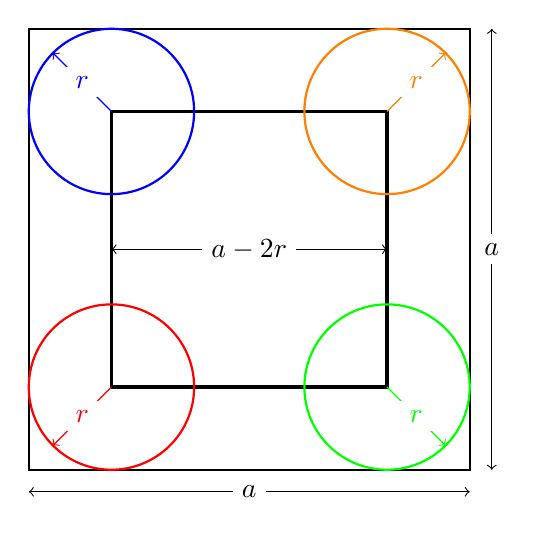
\begin{tikzpicture}[scale=.7]
\coordinate (c1) at (1.5,1.5);
\coordinate (c2) at (1.5,6.5);
\coordinate (c3) at (6.5,1.5);
\coordinate (c4) at (6.5,6.5);
\draw[very thick] (c1) -- (c3) -- (c4) -- (c2) -- cycle;
\draw[thick] (0,0) rectangle +(8,8);
\draw[color=red,thick] (c1) circle[radius=1.5];
\draw[color=blue,thick] (c2) circle[radius=1.5];
\draw[color=green,thick] (c3) circle[radius=1.5];
\draw[color=orange,thick] (c4) circle[radius=1.5];
\vertexcolor{c1}{red};
\vertexcolor{c2}{blue};
\vertexcolor{c3}{green};
\vertexcolor{c4}{orange};
\draw[<->] (0,-.4) -- node[fill=white] {$a$} (8,-.4);
\draw[<->] (8.4,0) -- node[fill=white] {$a$} (8.4,8);
\draw[->,red] (1.5,1.5) -- node[fill=white] {$r$} +(-135:1.5);
\draw[->,blue] (1.5,6.5) -- node[fill=white] {$r$} +(135:1.5);
\draw[->,green] (6.5,1.5) -- node[fill=white] {$r$} +(-45:1.5);
\draw[->,orange] (6.5,6.5) -- node[fill=white] {$r$} +(45:1.5);
\draw[<->] (1.5,4) -- node[fill=white] {$a-2r$} (6.5,4);
\end{tikzpicture}
\caption{Coins in a large square}\label{f.coins2}
\end{subfigure}
\end{center}
\end{figure}

\ans{2}
\[
E(\textsf{winnings per throw})=5\cdot\frac{1}{16}\,+\,(-1)\cdot\frac{15}{16}=-\frac{10}{16}=-0.625\,.
\]

\ans{3} \ref{f.coins2} shows four circles inscribed in the corners of the square. The side of the inner square is $a-2r$ so:
\[
P(\textsf{coin lands within the square})=\frac{(a-2r)^2}{a^2}\,.
\]
\sml{}
\begin{verbatim}
For side = 8, radius = 1:
Probability of landing within the square = 0.5625
Proportion landing within the square     = 0.5704
For side = 8, radius = 2:
Probability of landing within the square = 0.2500
Proportion landing within the square     = 0.2481
For side = 8, radius = 3:
Probability of landing within the square = 0.0625
Proportion landing within the square     = 0.0639
For side = 8, radius = 4:
Probability of landing within the square = 0.0000
Proportion landing within the square     = 0.0000
\end{verbatim}

%%%%%%%%%%%%%%%%%%%%%%%%%%%%%%%%%%%%%%%%%%%%%%%%%%%%%%%%%%%%%

\begin{prob}{Chuck-a-luck}
Choose number $n$ between $1$ and $6$ and throw three dice. If $n$ does not appear on any of the dice you lose $1$; if $n$ appears on one die you win $1$; if $n$ appears on two dice you win $2$; if $n$ appears on three dice you win $3$. What is the expectation of your winnings?
\end{prob}

\newpage

\solution{}

Let $P(k)$ be the probability that $n$ appears on $k$ dice. Then:
\[
E(\textsf{winnings per throw})=-1 P(0) + 1 P(1) + 2 P(2) + 3 P(3)\,.
\]
The throws of the three dice are independent so:
\begin{eqn}
E(\textsf{winnings per throw}) &=& 
-1 \dischoose{3}{0}\left(\frac{1}{6}\right)^0\left(\frac{5}{6}\right)^3
+1\dischoose{3}{1}\left(\frac{1}{6}\right)^1\left(\frac{5}{6}\right)^2+\\
&&\;\;\; 2{3\choose 2}\left(\frac{1}{6}\right)^2\left(\frac{5}{6}\right)^1+
3\dischoose{3}{3}\left(\frac{1}{6}\right)^3\left(\frac{5}{6}\right)^0\\
&=& \frac{1}{216}(-125+75+30+3)\approx -0.0787\,.
\end{eqn}%

\sml{}
\begin{verbatim}
Expectation of winnings = -0.0787
Average winnings        = -0.0724
\end{verbatim}

%%%%%%%%%%%%%%%%%%%%%%%%%%%%%%%%%%%%%%%%%%%%%%%%%%%%%%%%%%%%%

\begin{prob}{Curing the compulsive gambler}

\label{p.roulette}Roulette is a game played with a wheel having $38$ numbered pockets: $18$ red, $18$ black and $2$ green.\footnote{There are two green pockets in American roulette and one green pocket in European roulette.} The wheel is spun, a ball is thrown onto the wheel and you wait until the ball lands in one of the pockets. The ball lands in a random pocket with uniform distribution. You bet $1$ that the ball will land in a specific numbered (red or black) pocket.\footnote{This is the only type of bet used in the problems in this book.} If the ball lands in that pocket you receive $36$. Your net winnings are actually $35$ because the the $36$ includes the $1$ bet which is returned.

\que{1} What is the expectation your winnings if you play $36$ round of roulette?

\que{2} Your friend offers to bet you $20$ that after $36$ rounds you will have \emph{lost} money. What is the expectation of your winnings, taking into account the money won or lost both from the game and the bet with your friend?
\end{prob}

\solution{}

\ans{1} The probability of winning a single round is $1/38$ so:
\begin{eqn}
E(\textsf{winnings in one round})&=&35\cdot \frac{1}{38} + (-1)\cdot\frac{37}{38} = -\frac{2}{38} \approx -0.0526\\
E(\textsf{winnings in}\;36\;\textsf{rounds})&=&36\cdot -0.05266=-1.8947\,.
\end{eqn}%

\ans{2}
Consider the four outcomes of playing roulette for $36$ rounds:
\begin{itemize}
\item If you lose all the rounds you lose $36$.
\item If you win one round you win $35$ and you lose $35$ on the other rounds no money is won or lost.
\item If you win two rounds you win $70$ and you lose $34$ on the other rounds for a net win of $36$.
\item In general if you win $k$ rounds for $2<k\leq 36$ your net win is $35k - (36-k)>0$.
\end{itemize}
Therefore, you lose the bet only if you lose all rounds:
\begin{eqn}
P(\textrm{losing\ } 36 \textrm{\ rounds})&=&\left(\frac{37}{38}\right)^{36}\approx 0.3829\\
E(\textsf{total winnings})&=&\overbrace{-1.8947}^{\textsf{\small E of all rounds}}+\;\;
\overbrace{-20\cdot 0.3829}^{\textsf{\small lose bet}} \;+\; \overbrace{20\cdot (1-0.3829))}^{\textsf{\small win bet}} \approx 2.7904\,.
\end{eqn}%
Clearly you should take the bet!

\sml{}
\begin{verbatim}
Expectation of winning a round = -0.0526
Average winnings for a round   = -0.0593
\end{verbatim}
The simulation showed a large variance which was reduced by running one million trials.

%%%%%%%%%%%%%%%%%%%%%%%%%%%%%%%%%%%%%%%%%%%%%%%%%%%%%%%%%%%%%

\begin{prob}{Perfect bridge hand}
Randomly select $13$ cards from a deck. What is the probability that they will all be of the same suit?
\end{prob}

\solution{1}

There are $\dischoose{52}{13}$ ways of selecting $13$ cards from a deck of $52$ cards. Only four of them consist of $13$ cards from the same suit:
\[
P(\textsf{selecting}\;13\;\textsf{of same suit})=\frac{4}{\dischoose{52}{13}}=\frac{4\cdot 13!\cdot 39!}{52!}\approx 6.2991\times 10^{-12}\,.
\]

\solution{2}

There are $52$ ways of selecting the first card, then $12$ ways of selecting the second card of the same suit from the remaining $51$ cards, $11$ ways of selecting a third card, and so on:
\[
P(\textsf{selecting}\;13\;\textsf{cards of the same suit})=\frac{52}{52}\cdot \frac{12}{51}\cdot \frac{11}{50} \cdots  \frac{1}{40}= \frac{12!}{51!/39!}\approx 6.2991\times 10^{-12}\,.
\]

\newpage

\sml{}

There is no point in running a simulation with $52$ cards because the result would almost certainly be zero. A simulation was run with a deck of $16$ cards and $4$ suits.

\begin{verbatim}
Probability of perfect hand = 0.0022
Proportion perfect hand     = 0.0020
\end{verbatim}

%%%%%%%%%%%%%%%%%%%%%%%%%%%%%%%%%%%%%%%%%%%%%%%%%%%%%%%%%%%%%

\begin{prob}{Craps\annotate{D}}
Craps is a played with a pair of dice. On the first throw you win if the sum of the numbers is $7$ or $11$ and you lose if the sum is $2$, $3$ or $12$. If the sum on the first throw is $n=4,5,6,8,9,10$ (called a \emph{point}), continue to throw the dice until the sum is the point $n$ (a win) or $7$ (a loss).

\que{1} What are the probabilities of the following events on the first throw: winning, losing, neither winning nor losing?

\que{2} What is the probability of a win?
\end{prob}

\solution{1}

\ans{1} The outcome of throwing a die is uniformly distributed and the outcomes of throwing a pair of dice are independent, so the probability of any outcome is $1/36$. The number of ways of obtaining each of the events, the sum of a pair of dice, is:
\[
\begin{array}{l|rrrrrrrrrrr}
\textrm{Sum} & 2 & 3 & 4 & 5 & 6 & 7 & 8 & 9 & 10 & 11 & 12\\\hline
\textrm{Pairs} & 1 & 2 & 3 & 4 & 5 & 6 & 5 & 4 & 3 & 2 & 1
\end{array}
\]
On the first throw there are $8$ ways of throwing $7$ or $11$ so the probability of winning is $8/36$ and there are $4$ ways of throwing $2,3,12$ so the probability losing is $4/36$. The probability of neither winning nor losing on the first throw is:
\[
1 - \frac{8}{36} - \frac{4}{36} = \frac{24}{36}\,.
\]

%%%%%%%%%%%%%%%%%%%%%%%%%%%%%%%%%%%%

\ans{2}
Consider two cases:
\begin{itemize}
\item The point is $4$. The probability of winning on the second throw (a $4$) is $3/36$ and the probability of losing (a $7$) is $6/36$. The probability of neither winning nor losing is $1-(3/36)-(6/36)=27/36$.
\item The point is $8$. The probability of winning on the second throw (an $8$) is $5/36$ and the probability of losing (a $7$) is $6/36$. The probability of neither winning nor losing is $1-(5/36)-(6/36)=25/36$.
\end{itemize}
We see that the probability of winning must be computed separately for each of the points $4,5,6,8,9,10$, so we develop a general formula for the probability.

Let $P_n$ be the probability of winning by throwing the point $n$ on a throw and let $Q_n$ the probability of neither winning nor losing on a throw if the point is $n$. $W_n$, the probability of winning by \emph{eventually} throwing the point $n$ after the first throw, is computed by adding:
\begin{itemize}
\item The probability of throwing the point on the second throw.
\item The probability of neither winning nor losing on the second throw and throwing the point on the third throw.
\item The probability of neither winning nor losing on the second and third throws and throwing the point on the fourth throw,
\end{itemize}
and so on:
\begin{eqn}
W_n&=&P_n + Q_n P_n + Q_n^2 P_n+ Q_n^3 P_n  + \cdots\\
&=&P_n\left(1+Q_n^1 + Q_n^2+ Q_n^3  + \cdots\right)\\
&=&P_n\left(\frac{1}{1-Q_n}\right)\,.
\end{eqn}%
You lose on any throw after the first if you throw a $7$ with probability $6/36$ so:
\begin{eqn}
Q_n &=& (1-P_n)-(6/36)\\
W_n&=&\frac{P_n}{P_n+(6/36)}\,.
\end{eqn}%
$W_n$ for the six points are:
\[
\renewcommand{\arraystretch}{2}
\begin{array}{lcccccc}
n   & 4 & 5 & 6 & 8 & 9 & 10 \\\hline
P_n & \disfrac{3}{36} & \disfrac{4}{36} & \disfrac{5}{36} & \disfrac{5}{36} & \disfrac{4}{36} & \disfrac{3}{36} \\
%1-Q_n & \disfrac{9}{36} & \disfrac{10}{36} & \disfrac{11}{36} & \disfrac{11}{36} & \disfrac{10}{36} & \disfrac{9}{36} \\
W_n & \disfrac{3}{9} & \disfrac{4}{10} & \disfrac{5}{11} & \disfrac{5}{11} & \disfrac{4}{10} & \disfrac{3}{9}
\end{array}
\]
$W$, the probability of winning, can be computed by adding the probability of winning on the first throw to the sum of the probabilities for winning by throwing a point each multiplied by the probability of throwing \emph{that point} on the first throw:
\begin{equation}\label{eq.9-a}
W=\frac{8}{36}+\sum_{n\in\{4,5,6,8,9,10\}} P_nW_n \approx 0.4929\,.
\end{equation}
The casino's probability of winning a game of craps is
only $0.5-0.4929\approx 0.5\%$, but the law of large numbers ensures that they will eventually win and you will eventually lose!

%%%%%%%%%%%%%%%%%%%%%%%%%%%%%%%%%%%%

\newpage

\solution{2}

\ans{2} Consider the following sequences of throws where the point is $4$:
\[
\begin{array}{rrrrrrrrrrr}
4 & 8 & 9 & 9 & 9 & 8 & 8 & 8 & 9 & 8 & 4\\
4 & 8 & 9 & 9 & 9 & 8 & 8 & 8 & 9 & 8 & 7\\
4 & 9 & 9 & 9 & 8 & 8 & 4
\end{array}
\]
The games only terminates if a $4$ is thrown (win) or a $7$ is thrown (loss), so an appearance of an $8$ or a $9$ doesn't affect the result. Therefore, once a point has been thrown, the probability of winning is the conditional probability that a $4$ is thrown given that a $4$ or  a $7$ is thrown. Let $f$ be the event that a $4$ is thrown and $s$ be the event that a $7$ is thrown. Then:
\[
P(f|f\cup s) = \disfrac{P(f)\cap P(f\cup s)}{P(f\cup s)}=\disfrac{P(f)}{P(f\cup s)}=\disfrac{3/36}{(3+6)/36}=\disfrac{3}{9}\,,
\]
which is exactly the result $W_4$ in the table above. After computing $W_n$ for all points, Equation~\ref{eq.9-a} can be used to compute $W$.

Conditional probability is implicitly used in the first solution because $W_n$ is a probability that is conditional on the first throw resulting in the point $n$.

\sml{}
\begin{verbatim}
Probability of winning = 0.4929
Proportion of wins     = 0.4948
\end{verbatim}

%%%%%%%%%%%%%%%%%%%%%%%%%%%%%%%%%%%%%%%%%%%%%%%%%%%%%%%%%%%%%

\refstepcounter{problem}  % 10. An experiment in personal taste

%%%%%%%%%%%%%%%%%%%%%%%%%%%%%%%%%%%%%%%%%%%%%%%%%%%%%%%%%%%%%

\refstepcounter{problem}  % 11. Silent cooperation

%%%%%%%%%%%%%%%%%%%%%%%%%%%%%%%%%%%%%%%%%%%%%%%%%%%%%%%%%%%%%

\refstepcounter{problem}  % 12. Quo vadis?

%%%%%%%%%%%%%%%%%%%%%%%%%%%%%%%%%%%%%%%%%%%%%%%%%%%%%%%%%%%%%

\begin{prob}{The prisoner's dilemma}

Three prisoners $A,B,C$ are eligible for parole. The parole board will release two of them so the possibilities are $\{A,B\}, \{A,C\}, \{B,C\}$ with equal probability of $1/3$. Therefore, the probability that $A$ will be released is $2/3$. Prisoner $A$ is told correctly the name of  one of the other prisoners $B$ or $C$ who will be released. If $A$ is told that prisoner $B$ will be released, what is the probability that $A$ too will be released?
\end{prob}

The following three solutions are essentially the same but the methods of computing the conditional probabilities are somewhat different.

\solution{1}

There are four possible events (Figure~\ref{f.pp}):
\begin{description}
\item[$e_1$:] $A$ is told that $B$ will be released and $\{A,B\}$ are released. 
\item[$e_2$:] $A$ is told that $C$ will be released and $\{A,C\}$ are released. 
\item[$e_3$:] $A$ is told that $B$ will be released and $\{B,C\}$ are released. 
\item[$e_4$:] $A$ is told that $C$ will be released and $\{B,C\}$ are released. 
\end{description}
\begin{figure}[tb]
\begin{center}
\begin{tikzpicture}
\coordinate (root) at (0,0);
\draw[thick,->] (root) -- node[above] {$1/3$} (4,2)
  coordinate(top) node[right] {$\{B,C\}$};
\draw[thick,->] (root)-- node[above] {$1/3$} (4,0)
   coordinate(middle) node[right] {$\{A,B\}$};
\draw[thick,->] (root)-- node[below,yshift=-3pt] {$1/3$} (4,-2)
  coordinate(bottom) node[right]  {$\{A,C\}$};
\draw[thick,->] ($(top)+(1.6,0)$) --
  node[above] {$1/2$} +(4,.6)
  coordinate(one) node[right] {$B$};
\draw[thick,->] ($(top)+(1.6,0)$) --
  node[below] {$1/2$} +(4,-.6)
  coordinate(two) node[right] {$C$};
\draw[thick,->] ($(middle)+(1.6,0)$) --
  node[below] {$1$}  +(4,0) 
  coordinate(three) node[right] {$B$};
\draw[thick,->] ($(bottom)+(1.6,0)$) --
  node[below] {$1$} +(4,0)
  coordinate(four) node[right] {$C$};
\node at ($(top)+(.5,1.8)$) {Prisoners released};
\node at ($(one)+(.45,1.2)$) {$A$ told this prisoner released};
\end{tikzpicture}
\caption{Tree for the prisoner's dilemma}\label{f.pp}
\end{center}
\end{figure}
Each pair of prisoners has an equal probability of being released so:
\[
P(e_1)=P(e_2)=P(e_3\cup e_4)=\frac{1}{3}\,.
\]
If $\{B,C\}$ are to be released, $A$ is told correctly the name of either $B$ or $C$ who will be released and with equal probability, so $P(e_3)=P(e_4)=1/6$. The conditional probability that $A$ will be released (event $e_1$) given that $A$ is told that $B$ will be released ($e_1\cup e_3$) is:
\[
P(e_1|e_1\cup e_3) = \frac{P(e_1\cap(e_1\cup e_3))}{P(e_1\cup e_3)}=\frac{P(e_1)}{P(e_1\cup e_3)}=\frac{1/3}{(1/3)+(1/6)}=\frac{2}{3}\,.
\]

\solution{2}

The conditional probability that $A$ will be released given that $A$ that $B$ will be released is:
\[
P(A|B) = \frac{P(A\cap B)}{P(B)} = \frac{1/3}{2/3}=\frac{1}{2}\,.
\]
But this is \emph{not} the correct conditional probability. The new information is that $A$ is \emph{told} that $B$ will be released. Let $R_{AB}$ be the event that $A$ is told that $B$ will be released, then:
\[
P(A|R_{AB}) = \frac{P(A\cap R_{AB})}{P(R_{AB})}\,.
\]
The report of $B$'s release is true so:
\[
P(A\cap R_{AB})=P(\{A,B\})=\disfrac{1}{3}\,.
\]
If $\{B,C\}$ are to be released $A$ will be told that $B$ will be released with probability $1/2$ and also that $C$ will be released with probability $1/2$, so:
\begin{eqn}
P(R_{AB})&=&P(\{A,B\})+\disfrac{1}{2}\cdot P(\{B,C\})=\disfrac{1}{3}+\disfrac{1}{2}\cdot \disfrac{1}{3}=\disfrac{1}{2}\\
P(A|R_{AB})&=& \frac{P(A\cap R_{AB})}{P(R_{AB})} = \disfrac{1/3}{1/2}=\disfrac{2}{3}\,,
\end{eqn}

\solution{3}

$P(A)=2/3$ is given. $P(R_{AB}|A)=1/2$ because if $A$ is released, $B$ or $C$ will be released with equal probabilty. We have computed that $P(R_{AB})=1/2$. By Bayes' rule:
\[
P(A|R_{AB})= \frac{P(R_{AB}|A)\,P(A)}{P(R_{AB})} = \displaystyle\frac{(1/2)(2/3)}{1/2}=\displaystyle\frac{2}{3}\,.
\]

\begin{comment}
\textbf{\Large The Monty Hall problem}

\medskip

Here we present the Monty Hall problem (which does not appear in the book) in order to show the relation between it and the prisoner's dilemma problem.

Many discussions in the literature result from interpretations of the problem so in order to avoid confusion I will present in great detail the rules of the game and the assumptions that are sometimes left implicit:

\begin{enumerate}
\item In a television game show the contestant faces three closed doors. Behind each door is one surprise: a car and two goats.
\item The contestant prefers to win the car and not a goat.\footnote{I haven't found this implicit assumption mentioned in the literature but if we want to be precises it is worth uncovering.}
\item The position of each prize is random with a uniform distribution.
\item The host knows where each prize is.
\item The contestant must choose one door.
\item Before it is revealed to the contestant which prize he received, the host must open one of the doors with a goat. There are two possibilities:
\begin{itemize}
\item If the contestant chose the door with the car, the host's choice between the other two doors is random with uniform distribution.
\item If the contestant chose a door with a goat, the host must open the door with the second goat. 
\end{itemize}
After the door is opened the contestant must decide whether to stay with his original choice or to change it and choose the other unopened door.
\item The host opens the door that was chosen and the contestant wins the prize behind that door.
\end{enumerate}
What is the contestant's optimal strategy: to stay with the original door or to change his choice.

According to a common solution, the probability that the car is behind the original door changes from $1/3$ to $1/2$ because the car is behind one of the two remaining closed doors. Therefore, it doesn't matter whether the contestant stays with his original choice or changes it. This solution is \emph{not} correct because these aren't two independent trials. After opening the door, the host doesn't toss a coin to decide again where to place the car and where to place the goat.

Consider now a variation on the game where the contestant is \emph{not} allowed to change his choice! The probabilities don't change: he has a $1/3$ chance of winning the car and a $2/3$ chance of not winning. This is equivalent to the prisoner's dilemma problem because prisoner $A$ is not allowed to decide who is going to be released, so it doesn't matter what he is told. With the new rules it doesn't matter which door the host opens because the contestant can't do anything.

The Monty Hall problem is different. It is only because of the rule that the contestant is allowed to change his choice that opening the door has any meaning. Again, the probabilities don't change: there is a $1/3$ chance that the car is behind the door the contestant chose and a $2/3$ chance that it behind the other two doors. However, this $2/3$ is now ``concentrated'' in the one door that remains closed and, therefore, the contestant can double his chance of winning by changing his choice.

\sml{}


There is no simulation for the prisoner's dilemma problem because the problem asks if the probability changes as the result of some new data, but we have shown that there is no change. Here are the results of a simulation of the Monty Hall problem for $10000$ games:

\begin{verbatim}
Wins when staying with original door = 0.3311
Wins when changing door              = 0.6689
\end{verbatim}
\end{comment}

%%%%%%%%%%%%%%%%%%%%%%%%%%%%%%%%%%%%%%%%%%%%%%%%%%%%%%%%%%%%%

\begin{prob}{Collecting coupons}
Given a unbounded sequence of boxes each of which contains five coupons numbered $1$ to $5$, you randomly draw one coupon sequentially from each box.

\que{1} What is the expectation of the number of coupons drawn until you have all five of the numbers?

\que{2} Develop a formula for the expectation for $n$ numbers.

\textbf{Hint:} Use the solution to Problem~4 on page~\pageref{p.four} and the approximation for $H_n$, the sum of harmonic numbers (page~\pageref{p.harmonic}).
\end{prob}

\solution{}

\ans{1} What is the expectation of the number of draws until you get a  number that is \emph{different from} all the previous ones? By  Problem~4 this is $1/p$ where $p$ is the probability of drawing a different number. For the first draw the probability is $1$ so the expectation is $1=5/5$, for the second draw the probability is $4/5$ so expectation is $5/4$, and so on. Therefore:
\[
E(\textsf{all five numbers}) = \frac{5}{5}+\frac{5}{4} + \frac{5}{3} + \frac{5}{2} + \frac{5}{1} = \frac{}{} =\frac{1370}{120}\approx 11.4167\,.
\]
\ans{2} Use the same method and the approximation for $H_n$:
\[
E(\textsf{all}\;n \;\textsf{numbers}) = n\left(\frac{1}{n}+\frac{1}{n-1} + \cdots \frac{1}{2} + \frac{1}{1}\right) =nH_n\approx n\left(\ln n + \frac{1}{2n} + 0.5772\right)\,. 
\]
For $n=5$ this gives:
\[
E(\textsf{all five numbers}) =5H_5\approx 5\left(\ln 5 + \frac{1}{10} + 0.5772\right) \approx 11.4332\,.
\]

\newpage

\sml{}
\begin{verbatim}
For  5 coupons:
Expectation of draws = 11.4332
Average draws        = 11.3339
For 10 coupons:
Expectation of draws = 29.2979
Average draws        = 29.3001
For 20 coupons:
Expectation of draws = 71.9586
Average draws        = 71.6250
\end{verbatim}

%%%%%%%%%%%%%%%%%%%%%%%%%%%%%%%%%%%%%%%%%%%%%%%%%%%%%%%%%%%%%

\begin{prob}{The theater row}
Arrange $8$ even numbers and $7$ odd numbers randomly in a row, for example:
\[
10\quad 12\quad 3\quad 2\quad 9\quad 6 \quad 1\quad 13\quad 7\quad 10\quad 3\quad 8\quad 8\quad 5\quad 20\,,
\]
which we can write as follows since the specific numbers are not important:
\[
E\quad E\quad O\quad E\quad O\quad E \quad O\quad O\quad O\quad E\quad O\quad E\quad E\quad O\quad E\,.
\]
What is the expectation of the number of even-odd or odd-even adjacent pairs?

In the example there are $10$ $EO$ or $OE$ adjacent pairs.

\textbf{Hint:} What is the probability that a pair of adjacent number are different?
\end{prob}

\solution{}

The following table shows the $10$ possible arrangements of $3$ even and $2$ odd numbers. The total number of different adjacent pairs is $24$ and the average is $24/10=2.4$.
\[
\begin{array}{l|r@{\hspace{2em}}|@{\hspace{2pt}}|@{\hspace{2em}}l|r}
\textsf{Arrangement}&\textsf{Pairs}&\textsf{Arrangement}&\textsf{Pairs}\\\hline
EEEOO & 1&
EEOEO & 3\\
EEOOE & 2&
EOEOE & 4\\
EOEEO & 3&
EOOEE & 2\\
OEEOE & 3&
OEEEO & 2\\
OEOEE & 3&
OOEEE & 1\\
\end{array}
\]
Returning to the example with $15$ numbers, let $P_d$ be the probability that a given pair in an arrangement is $EO$ or $OE$:
\[
P_d =P(EO) + P(OE) = \frac{8}{15}\cdot \frac{7}{14} + \frac{7}{15}\cdot \frac{8}{14} = 2\cdot \frac{8}{15}\cdot \frac{7}{14} = \frac{8}{15}\,.
\]
Let $E_d$ be the expectation of the number of pairs in an arrangement that are $EO$ or $OE$. Since an $EO$ or $OE$ pair contributes $1$ to the count of different pairs and an $EE$ or an $OO$ pair contributes $0$:
\[
E_d =
\sum_{\textsf{\footnotesize all pairs}} (1\cdot P_d + 0\cdot (1-P_d))= 14\cdot \frac{8}{15} \approx 7.4667\,.
\]

Check for $10$ numbers:
\begin{eqn}
P_d &=& P(EO) + P(OE) = \frac{3}{5}\cdot \frac{2}{4} + \frac{2}{5}\cdot \frac{3}{4} = \frac{3}{5}\\
E_d &=& 4\cdot \frac{3}{5}=\frac{12}{5}=2.4\,.
\end{eqn}%

\sml{}
\begin{verbatim}
For  5 places:
Expectation of different pairs = 2.4000
Average different pairs        = 2.3855
For 15 places:
Expectation of different pairs = 7.4667
Average different pairs        = 7.4566
For 27 places:
Expectation of different pairs = 13.4815
Average different pairs        = 13.4835
For 49 places:
Expectation of different pairs = 24.4898
Average different pairs        = 24.4725
\end{verbatim}

%%%%%%%%%%%%%%%%%%%%%%%%%%%%%%%%%%%%%%%%%%%%%%%%%%%%%%%%%%%%%

\begin{prob}{Will the second-best be runner-up?}
Eight players $\{a_1,\ldots,a_8\}$ are randomly assigned to play eight games $\{g_1,\ldots,g_8\}$ in a tournament such that player $a_{k_i}$ plays his first game in place $g_i$ (Figure~\ref{f.tournament}). The players are ranked from the best $a_1$ to the worst $a_8$ and the better player will \emph{always} defeat his opponent.  Clearly $a_1$ will win the tournament.

\que{1} What is the probability that $a_2$ will be the runner-up by playing $a_1$ in the final round and losing?

\que{2} If there are $2^n$ players what is the probability that $a_2$ will be the runner-up by playing $a_1$ in the final round and losing?
\begin{figure}[tb]
\begin{center}
\begin{tikzpicture}[scale=.75]
\foreach \n in {1,2,3,4,5,6,7,8}
  \node (\n) at (0,\n*10mm) {$g_{\n}:$};
\foreach \n in {1,2,3,4}
  \node[inner sep=-4pt] (r\n) at (40mm,-5mm+\n*20mm) {};
\foreach \n/\r in {1/1,2/1,3/2,4/2,5/3,6/3,7/4,8/4}
  \draw (\n) --
     node[very near start,fill=white] {$a_{k_{\n}}$} +(30mm,0)
     -- ($(r\r)+(1pt,0)$);
\foreach \n/\v in {1/25mm,2/65mm}
  \node[inner sep=-5pt] (rr\n) at (70mm,\v) {};
\foreach \n/\r in {1/1,2/1,3/2,4/2}
  \draw ($(r\n)+(1pt,0)$) -- ++(21mm,0) -- 
  ($(rr\r)+(-1pt,0)$) -- ++(20mm,0);
\node[inner sep=-5pt] (rrr) at ($(rr1)+(40mm,22.5mm)$) {};
\foreach \n/\r in {1,2}
 \draw ($(rr\n)+(19.6mm,0)$) -- ($(rrr)+(1pt,0)$); 
\draw ($(rrr)+(1pt,0)$) -- +(40mm,0);
\node at (32mm,88mm) {\textsf{\small Quarterfinals}};
\node at (62mm,88mm) {\textsf{\small Semifinals}};
\node at (90mm,88mm) {\textsf{\small Final}};
\end{tikzpicture}
\end{center}
\caption{A tournament schedule}\label{f.tournament}
\end{figure}
\end{prob}

\solution{}

\ans{1}
If $a_1$ is assigned to one of the games $\{g_1,g_2,g_3,g_4\}$ none of the other players assigned to these games will reach the final, so $a_2$ must be assigned to one of $\{g_5,g_6,g_7,g_8\}$. The temptation is to conclude that the probability of $a_2$ being the runner-up is $1/2$ since $a_2$ must be assigned to one of the four games $\{g_1,g_2,g_3,g_4\}$. However, whatever game $a_1$ is  assigned to, $a_2$ will be the runner up only if he is assigned to one of the four \emph{remaining} seven games so the probability is $4/7$.

\ans{2} Similarly, of the $2^n-1$ games that $a_1$ is not assigned to, $a_2$ must be assigned to one of the $2^{n-1}$ games not in the same half as $a_1$. Therefore:
\[
P(a_1,a_2\;\textsf{playing each other in the final})=\frac{2^{n-1}}{2^n-1}\,.
\]

\sml{}
\begin{verbatim}
For   8 players:
Probability a2 is runner-up                = 0.5714
Proportion of games where a2 is runner-up  = 0.5707
For  32 players:
Probability a2 is runner-up                = 0.5161
Proportion of games where a2 is runner-up  = 0.5184
For 128 players:
Probability a2 is runner-up                = 0.5039
Proportion of games where a2 is runner-up  = 0.5060
\end{verbatim}

%%%%%%%%%%%%%%%%%%%%%%%%%%%%%%%%%%%%%%%%%%%%%%%%%%%%%%%%%%%%%

\newpage

\begin{prob}{Twin knights\annotate{D}}

Eight players $\{a_1,\ldots,a_8\}$ are randomly assigned to play games $\{g_1,\ldots,g_8\}$ in a tournament (Figure~\ref{f.tournament}). Let $P(i,j)$ be the probability that $a_i$ wins against $a_j$. For all $i,j$, $P(i,j)=P(j,i)=1/2$.

\que{1} What is the probability that $a_1,a_2$ play each other?

\que{2} If there are $2^n$ players what is the probability that $a_1,a_2$ play each other?
\end{prob}

\solution{}

\ans{1} Without loss of generality assign $a_1$ to $g_1$. Consider the different possibilities that $a_1,a_2$ play each other. With probability $1/7$, $a_2$ is assigned to $g_2$. With probability $2/7$, $a_2$ is assigned to $g_3$ or $g_4$, but $a_2$ doesn't play $a_1$ unless \emph{both} of them win their first game, so we need to multiply the probability of this assignment by $1/4$. With probability $4/7$, $a_2$ is assigned to $g_5,g_6,g_7,g_8$, but $a_2$ doesn't play $a_1$ unless \emph{both} of them win their first two  games, so we need to multiply the probability of this assignment by $1/16$. Therefore:
\[
P(a_1, a_2\;\textsf{play each other})=\frac{1}{7} + \frac{1}{4}\cdot \frac{2}{7} + \frac{1}{16}\cdot \frac{4}{7} =\frac{1}{4}\,.
\]

\ans{2}
Let $P_n$ be the probability that in a tournament with $2^n$ players $a_1$ and $a_2$ play each other. We have shown that $P_3=1/4$. What about $P_4$? Using the same approach:
\begin{eqn}
P_4 &=& \frac{1}{15} + \frac{1}{4}\cdot \frac{2}{15}  + \frac{1}{16}\cdot \frac{4}{15}  + \frac{1}{64}\cdot \frac{8}{15} \\
&=&\frac{1}{15}\left(1+\frac{1}{2}+\frac{1}{4}+\frac{1}{8}\right)=\frac{1}{8}\,.
\end{eqn}%
It is reasonable to conjecture that $P_n=1/2^{n-1}$.

\textbf{Proof 1:} Using the same approach and the formula for the sum of a geometric series:
\begin{eqn}
P_n&=&\frac{1}{2^n-1}\sum_{i=0}^{n-1}2^i\cdot \left(\frac{1}{2}\right)^{2i}\\
&=&\frac{1}{2^n-1}\sum_{i=0}^{n-1}2^{-i}\\
&=&\frac{1}{2^n-1}
  \left(
    \frac{1-(1/2)^{(n-1)+1}}
         {1-(1/2)}
  \right)=\frac{1}{2^{n-1}}\,.
\end{eqn}%

\textbf{Proof 2:} By induction. The base case is $P_3=1/4=1/2^{3-1}$.

There are two inductive steps:

\textit{Case 1:} $a_1$ and $a_2$ are assigned to different halves of the tournament:
\[
P(a_1,a_2\;\textsf{assigned to different halves})=\frac{2^{n-1}}{2^n-1}\,.
\]
They can only meet in the final game and therefore both must win all of their $n-1$ games:
\begin{equation}\label{eq.17a}
P(a_1,a_2\;\textsf{meet if assigned to different halves})=\frac{2^{n-1}}{2^n-1} \left(\frac{1}{2}\right)^{n-1} \left(\frac{1}{2}\right)^{n-1}=\frac{2^{-(n-1)}}{2^n-1}\,.
\end{equation}
\textit{Case 2:} $a_1$ and $a_2$ are assigned to the same half of the tournament:
\[
P(a_1,a_2\;\textsf{assigned to the same half})=\frac{2^{n-1}-1}{2^n-1}\,.
\]
Since both players are in the same half the problem has been reduced to determining $P_{n-1}$. By the inductive hypothesis:
\begin{equation}\label{eq.17b}
P(a_1,a_2\;\textsf{meet if assigned to the same half})=\frac{2^{n-1}-1}{2^n-1}\cdot \frac{1}{2^{n-2}}=\frac{2^{1}-2^{-(n-2)}}{2^n-1}\,.
\end{equation}
Combining Equations~\ref{eq.17a}, \ref{eq.17b} gives:
\[
\renewcommand*{\arraystretch}{2.2}
\begin{array}{rcl}
P_n&=&\disfrac{2^{-(n-1)}}{2^n-1}+\disfrac{2^{1}-2^{-(n-2)}}{2^n-1}\\
&=&\disfrac{2^{n-1}}
        {2^{n-1}}\cdot 
   \disfrac{2^{-(n-1)}+2^{1}-2^{-(n-2)}}
        {2^n-1}\\
&=&\disfrac{1}
        {2^{n-1}}\cdot 
   \disfrac{2^0+2^n-2^1}
        {2^n-1}=\disfrac{1}{2^{n-1}}\,.
\end{array}
\]

\sml{}
\begin{verbatim}
For   8 players:
Probability that a1, a2 meet = 0.2500
Proportion a1, a2 meet       = 0.2475
For  32 players:
Probability that a1, a2 meet = 0.0625
Proportion a1, a2 meet       = 0.0644
For 128 players:
Probability that a1, a2 meet = 0.0156
Proportion a1, a2 meet       = 0.0137
\end{verbatim}

%%%%%%%%%%%%%%%%%%%%%%%%%%%%%%%%%%%%%%%%%%%%%%%%%%%%%%%%%%%%%

\begin{prob}{An even split at coin tossing}
\que{1} Toss a fair coin $20$ times. What is the probability of obtaining $10$ heads?

\que{2} Toss a fair coin $40$ times. What is the probability of obtaining $20$ heads?
\end{prob}

\newpage

\solution{}

\ans{1} Since the coin is fair the probability of obtaining $10$ heads in $20$ tosses is given by the binomial distribution:
\[
P(10\;\textsf{heads in}\; 20\; \textsf{tosses})={20 \choose 10} \left(\frac{1}{2}\right)^{10}\left(\frac{1}{2}\right)^{10} \approx 0.1762\,.
\]

\ans{2} You might expect the probability to be the same before but:
\[
P(20\;\textsf{heads in}\; 40\; \textsf{tosses})={40 \choose 20} \left(\frac{1}{2}\right)^{20}\left(\frac{1}{2}\right)^{20}\approx 0.1254\,.
\]
By the law of large numbers the numbers of heads and tails will be ``roughly'' equal \cite[Section~8.4]{ross}, but they are unlikely to be exactly the same, and this event becomes less likely as the number of tosses increases.

\sml{}
\begin{verbatim}
Probability of 10 heads for  20 tosses = 0.1762
Proportion  of 10 heads for  20 tosses = 0.1790
Probability of 20 heads for  40 tosses = 0.1254
Proportion  of 20 heads for  40 tosses = 0.1212
Probability of 50 heads for 100 tosses = 0.0796
Proportion  of 50 heads for 100 tosses = 0.0785
\end{verbatim}

%%%%%%%%%%%%%%%%%%%%%%%%%%%%%%%%%%%%%%%%%%%%%%%%%%%%%%%%%%%%%

\begin{prob}{Isaac Newton helps Samuel Pepys}
\que{1} What is the probability of obtaining \emph{at least one} $6$ when $6$ dice are thrown?

\que{2} What is the probability of obtaining \emph{at least two} $6$'s when $12$ dice are thrown?

\que{3} Develop a formula for the probability of obtaining at least $n$ $6$'s when $6n$ dice are thrown.
\end{prob}

\solution{}

\ans{1} The probability is the complement of the probability of obtaining zero $6$'s in $6$ throws:
\[
P(\textsf{at least one}\; 6)=1-\left(\frac{5}{6}\right)^6\approx 0.6651\,.
\]

\ans{2} The probability is the complement of the probability of obtaining zero or one $6$'s in $12$ throws:
\[
P(\textsf{at least two}\;6\textsf{s})=1-\left(\frac{5}{6}\right)^{12}-{12\choose 1}\left(\frac{1}{6}\right)^{1}\left(\frac{5}{6}\right)^{11}\approx 0.6187\,.
\]
This event is less probable than the previous one.

\ans{3} The probability is the complement of the probability of obtaining less than $n$ $6$'s in $6n$ throws:
\begin{eqn}
P(\textsf{at least}\;n\;6\textsf{s})&=&
  1-{6n \choose 0}\left(\frac{1}{6}\right)^0\left(\frac{5}{6}\right)^{6n-0}-
  {6n\choose 1}\left(\frac{1}{6}\right)^{1}\left(\frac{5}{6}\right)^{6n-1}-\cdots\\
&=&1-\sum_{i=0}^{n-1}{6n\choose i}\left(\frac{1}{6}\right)^{i}\left(\frac{5}{6}\right)^{6n-i}\,.
\end{eqn}%

\sml{}
\begin{verbatim}
For   6 dice to throw  1 sixes:
Probability = 0.6651
Proportion  = 0.6566
For  12 dice to throw  2 sixes:
Probability = 0.6187
Proportion  = 0.6220
For  18 dice to throw  3 sixes:
Probability = 0.5973
Proportion  = 0.5949
For  96 dice to throw 16 sixes:
Probability = 0.5424
Proportion  = 0.5425
For 360 dice to throw 60 sixes:
Probability = 0.5219
Proportion  = 0.5250
\end{verbatim}

%%%%%%%%%%%%%%%%%%%%%%%%%%%%%%%%%%%%%%%%%%%%%%%%%%%%%%%%%%%%%

\begin{prob}{The three-cornered duel\annotate{D}}
$A,B,C$ fight a sequence of duels. Each of them has a fixed probability of winning a duel regardless of who the opponent is:
\[
P(A)=0.3,\quad P(B)=1, \quad P(C)=0.5\,.
\]
A person who is hit no longer participates in the duels. The shots are fired one at a time sequentially in the order $A,B,C$. If two opponents are still standing the shooter can decide whom to fire at. Assume that each person makes the optimal decision for each duel.

\que{1} What is $A$'s best strategy?

\que{2} Suppose that $A$ fires the first shot into the air. Is this a better strategy?

\textbf{Hint:} Give a formal definition for one strategy is better than another.

\textbf{Hint:} Compute the conditional probabilities of $A$ winning depending on whether $A$ chooses to shoot first at $B$ or $C$.
\end{prob}

\solution{}

Let $I_X$ be the indicator variable for $X$ winning the sequence of duels:
\[
I_X=
\left\{
\begin{array}{ll}
1,\quad X\;\textsf{wins the sequence of duels}\\
0, \quad X\; \textsf{loses the sequence of duels}\,.
\end{array}
\right.
\]
Strategy $s_1$ for $X$ is better strategy $s_2$ if the expectation of $I_X$ is greater for $s_1$ than for $s_2$.

Notation: \duel{X}{H}{Y} denotes that $X$ shoots at $Y$ and hits. \duel{X}{M}{Y} denotes that $X$ shoots at $Y$ and misses.

\ans{1}
Compute the conditional probabilities of $A$ winning.

\textit{Case 1:} $A$ chooses to shoot first at $C$.

If \duel{A}{M}{C} (probability $0.7$) then \duel{B}{H}{C} since $C$ is more dangerous than $A$. $A$ now shoots again at $B$ with probability $0.3$ of hitting, but if $A$ misses then \duel{B}{H}{A} with probability $1$ and $A$ loses.

If \duel{A}{H}{C} (probability $0.3$) then \duel{B}{H}{A} with probability $1$ and $A$ loses.

\vspace*{-3ex}
\[
\renewcommand*{\arraystretch}{2.5}
\begin{array}{l}
E(A \;\textsf{wins}\;|A\;\textsf{chooses to shoot first at}\;C) =\\
%
\qquad\quad \overbrace{1\cdot (0.7\cdot 1 \cdot 0.3)}^%
{\duelmath{A}{M}{C}, \duelmath{B}{H}{C}, \duelmath{A}{H}{B}}\; +
%
\overbrace{0\cdot (0.7\cdot 1\cdot 0.7\cdot 1)}^%
{\duelmath{A}{M}{C},  \duelmath{B}{H}{C}, \duelmath{A}{M}{B}, \duelmath{B}{H}{A}}+
%
\;\;\overbrace{0\cdot (0.3\cdot 1)}^%
{\duelmath{A}{H}{C}, \duelmath{B}{H}{A}}=0.2100\,.
\end{array}
\]
\textit{Case 2:} $A$ chooses to shoot first at $B$.

If \duel{A}{M}{B} (probability $0.7$) then as before \duel{B}{H}{C} and $A$ has one more chance to hit $B$ (probability $0.3$), otherwise \duel{B}{H}{A} with probability $1$ and $A$ loses.

If \duel{A}{H}{B} (probability $0.3$) then $A,C$ alternately shoot at each other until one is hit. The possibilities are:
\[
\begin{array}{ll}
(1)&C\stackrel{H}{\longrightarrow}A\\
(2)&C\stackrel{M}{\longrightarrow}A \stackrel{H}{\longrightarrow}C\\
(3)&C\stackrel{M}{\longrightarrow}A \stackrel{M}{\longrightarrow}C\stackrel{H}{\longrightarrow}A\\
(4)&C\stackrel{M}{\longrightarrow}A \stackrel{M}{\longrightarrow}C\stackrel{M}{\longrightarrow}A\stackrel{H}{\longrightarrow}C\\
(5)&C\stackrel{M}{\longrightarrow}A \stackrel{M}{\longrightarrow}C\stackrel{M}{\longrightarrow}A\stackrel{M}{\longrightarrow}C\stackrel{H}{\longrightarrow}A\\
(6)&C\stackrel{M}{\longrightarrow}A \stackrel{M}{\longrightarrow}C\stackrel{M}{\longrightarrow}A\stackrel{M}{\longrightarrow}C\stackrel{M}{\longrightarrow}A\stackrel{H}{\longrightarrow}C\\
&\cdots
\end{array}
\]
The probability of $A$ wins by eventually hitting $C$ is the sum of the probabilities of the even-numbered scenarios in the list:
\begin{eqn}
P(A\;\textsf{wins} \;| A\; \textsf{hits}\;B )&=&(0.5 \cdot 0.3) + \\
&&(0.5 \cdot 0.7) (0.5 \cdot 0.3) + \\
&&(0.5 \cdot 0.7) (0.5 \cdot 0.7) (0.5 \cdot 0.3)+ \cdots\\
&=&0.15 \sum_{i=0}^{\infty} 0.35^i= \frac{0.15}{1-0.35}=\frac{3}{13}\approx 0.2308\,.
\end{eqn}%
Similarly, the probability of $C$ winning is $\disfrac{0.5}{1-0.35}=\disfrac{10}{13}\approx 0.7692$.

The expectation is:
\vspace*{-1ex}
\[
\renewcommand*{\arraystretch}{1.5}
\begin{array}{l}
E(A \;\textsf{wins}) =E(A \;\textsf{wins}\;|\;A\;\textsf{misses}\;B) + E(A \;\textsf{wins}\;|\;A\;\textsf{hits}\;B)=\\
\qquad\qquad
\overbrace{1\cdot (0.7\cdot 1\cdot 0.3)}%
^{A\stackrel{M}{\longrightarrow}B, B\stackrel{H}{\longrightarrow}C, A\stackrel{H}{\longrightarrow}B}\;+
%
\overbrace{0\cdot (0.7\cdot 1\cdot 0.7\cdot 1)}%
^{A\stackrel{M}{\longrightarrow}B,
B\stackrel{H}{\longrightarrow}C,
A\stackrel{M}{\longrightarrow}B,
B\stackrel{H}{\longrightarrow}A}\; +
%
\overbrace{1\cdot 0.2308}%
^{A\stackrel{H}{\longrightarrow}B,
C\stackrel{H}{\longleftrightarrow*}A,
A\stackrel{H}{\longrightarrow}C}\; +\\
%
\qquad\;\,\overbrace{0\cdot 0.7692}%
^{A\stackrel{H}{\longrightarrow}B,
C\stackrel{H}{\longleftrightarrow*}A,
C\stackrel{H}{\longrightarrow}A}
\approx \; 0.2792\,,
\end{array}
\]
which is higher than the expectation of winning by shooting at $C$ first.

\ans{2} If $A$ shoots into the air not hitting anyone (probability $1$) then $B\stackrel{H}{\longrightarrow}C$ with probability $1$ and $A$ can try to hit $B$ with probability $0.3$. The expectation is:
\[
E(A \;\textsf{wins}|A\;\textsf{shoots in the air}) = 1\cdot (1\cdot 1 \cdot 0.3) + 0\cdot(1\cdot 1\cdot 0.7)=0.3\,,
\]
which is higher than the expectation for the other two strategies!

\sml{}
\begin{verbatim}
For A fires first at C:
Expectation of wins = 0.2100
Average wins        = 0.2138
For A fires first at B:
Expectation of wins = 0.2792
Average wins        = 0.2754
For A fires in the air:
Expectation of wins = 0.3000
Average wins        = 0.3000
\end{verbatim}

%%%%%%%%%%%%%%%%%%%%%%%%%%%%%%%%%%%%%%%%%%%%%%%%%%%%%%%%%%%%%
